% Options for packages loaded elsewhere
\PassOptionsToPackage{unicode}{hyperref}
\PassOptionsToPackage{hyphens}{url}
\PassOptionsToPackage{dvipsnames,svgnames,x11names}{xcolor}
%
\documentclass[
  letterpaper,
  DIV=11,
  numbers=noendperiod]{scrartcl}

\usepackage{amsmath,amssymb}
\usepackage{iftex}
\ifPDFTeX
  \usepackage[T1]{fontenc}
  \usepackage[utf8]{inputenc}
  \usepackage{textcomp} % provide euro and other symbols
\else % if luatex or xetex
  \usepackage{unicode-math}
  \defaultfontfeatures{Scale=MatchLowercase}
  \defaultfontfeatures[\rmfamily]{Ligatures=TeX,Scale=1}
\fi
\usepackage{lmodern}
\ifPDFTeX\else  
    % xetex/luatex font selection
\fi
% Use upquote if available, for straight quotes in verbatim environments
\IfFileExists{upquote.sty}{\usepackage{upquote}}{}
\IfFileExists{microtype.sty}{% use microtype if available
  \usepackage[]{microtype}
  \UseMicrotypeSet[protrusion]{basicmath} % disable protrusion for tt fonts
}{}
\makeatletter
\@ifundefined{KOMAClassName}{% if non-KOMA class
  \IfFileExists{parskip.sty}{%
    \usepackage{parskip}
  }{% else
    \setlength{\parindent}{0pt}
    \setlength{\parskip}{6pt plus 2pt minus 1pt}}
}{% if KOMA class
  \KOMAoptions{parskip=half}}
\makeatother
\usepackage{xcolor}
\setlength{\emergencystretch}{3em} % prevent overfull lines
\setcounter{secnumdepth}{-\maxdimen} % remove section numbering
% Make \paragraph and \subparagraph free-standing
\makeatletter
\ifx\paragraph\undefined\else
  \let\oldparagraph\paragraph
  \renewcommand{\paragraph}{
    \@ifstar
      \xxxParagraphStar
      \xxxParagraphNoStar
  }
  \newcommand{\xxxParagraphStar}[1]{\oldparagraph*{#1}\mbox{}}
  \newcommand{\xxxParagraphNoStar}[1]{\oldparagraph{#1}\mbox{}}
\fi
\ifx\subparagraph\undefined\else
  \let\oldsubparagraph\subparagraph
  \renewcommand{\subparagraph}{
    \@ifstar
      \xxxSubParagraphStar
      \xxxSubParagraphNoStar
  }
  \newcommand{\xxxSubParagraphStar}[1]{\oldsubparagraph*{#1}\mbox{}}
  \newcommand{\xxxSubParagraphNoStar}[1]{\oldsubparagraph{#1}\mbox{}}
\fi
\makeatother


\providecommand{\tightlist}{%
  \setlength{\itemsep}{0pt}\setlength{\parskip}{0pt}}\usepackage{longtable,booktabs,array}
\usepackage{calc} % for calculating minipage widths
% Correct order of tables after \paragraph or \subparagraph
\usepackage{etoolbox}
\makeatletter
\patchcmd\longtable{\par}{\if@noskipsec\mbox{}\fi\par}{}{}
\makeatother
% Allow footnotes in longtable head/foot
\IfFileExists{footnotehyper.sty}{\usepackage{footnotehyper}}{\usepackage{footnote}}
\makesavenoteenv{longtable}
\usepackage{graphicx}
\makeatletter
\newsavebox\pandoc@box
\newcommand*\pandocbounded[1]{% scales image to fit in text height/width
  \sbox\pandoc@box{#1}%
  \Gscale@div\@tempa{\textheight}{\dimexpr\ht\pandoc@box+\dp\pandoc@box\relax}%
  \Gscale@div\@tempb{\linewidth}{\wd\pandoc@box}%
  \ifdim\@tempb\p@<\@tempa\p@\let\@tempa\@tempb\fi% select the smaller of both
  \ifdim\@tempa\p@<\p@\scalebox{\@tempa}{\usebox\pandoc@box}%
  \else\usebox{\pandoc@box}%
  \fi%
}
% Set default figure placement to htbp
\def\fps@figure{htbp}
\makeatother

\usepackage{booktabs}
\usepackage{longtable}
\usepackage{array}
\usepackage{multirow}
\usepackage{wrapfig}
\usepackage{float}
\usepackage{colortbl}
\usepackage{pdflscape}
\usepackage{tabu}
\usepackage{threeparttable}
\usepackage{threeparttablex}
\usepackage[normalem]{ulem}
\usepackage{makecell}
\usepackage{xcolor}
\KOMAoption{captions}{tableheading}
\makeatletter
\@ifpackageloaded{caption}{}{\usepackage{caption}}
\AtBeginDocument{%
\ifdefined\contentsname
  \renewcommand*\contentsname{Table of contents}
\else
  \newcommand\contentsname{Table of contents}
\fi
\ifdefined\listfigurename
  \renewcommand*\listfigurename{List of Figures}
\else
  \newcommand\listfigurename{List of Figures}
\fi
\ifdefined\listtablename
  \renewcommand*\listtablename{List of Tables}
\else
  \newcommand\listtablename{List of Tables}
\fi
\ifdefined\figurename
  \renewcommand*\figurename{Figure}
\else
  \newcommand\figurename{Figure}
\fi
\ifdefined\tablename
  \renewcommand*\tablename{Table}
\else
  \newcommand\tablename{Table}
\fi
}
\@ifpackageloaded{float}{}{\usepackage{float}}
\floatstyle{ruled}
\@ifundefined{c@chapter}{\newfloat{codelisting}{h}{lop}}{\newfloat{codelisting}{h}{lop}[chapter]}
\floatname{codelisting}{Listing}
\newcommand*\listoflistings{\listof{codelisting}{List of Listings}}
\makeatother
\makeatletter
\makeatother
\makeatletter
\@ifpackageloaded{caption}{}{\usepackage{caption}}
\@ifpackageloaded{subcaption}{}{\usepackage{subcaption}}
\makeatother

\usepackage{bookmark}

\IfFileExists{xurl.sty}{\usepackage{xurl}}{} % add URL line breaks if available
\urlstyle{same} % disable monospaced font for URLs
\hypersetup{
  pdftitle={Analysis of International Education Costs vs.~University Rankings},
  pdfauthor={Girika; Chen Liu; Chang Heng-Hsieh},
  colorlinks=true,
  linkcolor={blue},
  filecolor={Maroon},
  citecolor={Blue},
  urlcolor={Blue},
  pdfcreator={LaTeX via pandoc}}


\title{Analysis of International Education Costs vs.~University
Rankings}
\author{Girika \and Chen Liu \and Chang Heng-Hsieh}
\date{}

\begin{document}
\maketitle


\subsection{Executive Summary}\label{executive-summary}

This comprehensive study examines the relationship between international
education costs and university rankings across the top 10 QS-ranked
countries for Master's degree programs. Our analysis reveals no direct
correlation between academic prestige and affordability, challenging
common assumptions about premium education pricing.

\subsection{Introduction}\label{introduction}

The international education sector is growing rapidly, with more
students exploring study opportunities beyond their home countries in
search of both quality and affordability. The QS World University
Rankings serve as a trusted benchmark for comparing institutions across
dimensions such as academic reputation, graduate employability, and
sustainability. \textbf{While top-ranked universities typically involve
higher costs, the total expense varies significantly between countries
due to differences in living costs, visa requirements, and local
economic conditions.}

For many prospective students, cost considerations are just as critical
as academic quality when making study abroad decisions. However, limited
research has systematically compared education costs across top-ranking
university destinations, making it difficult for students to make
informed decisions about cost-effective study options. This study
addresses this knowledge gap by examining both academic performance and
financial affordability through merging QS ranking data from 2024 and
2025 with international education cost datasets. Our analysis focuses
specifically on master's degree programs in the top 10 countries with
the highest QS university rankings. We calculate total study costs
including tuition, accommodation, visa fees, and insurance to provide
comprehensive cost comparisons. The findings aim to provide practical
guidance for international students seeking optimal value in their
education investment.

\subsection{Methodology}\label{methodology}

\textbf{Research Design and Data Sources}

This study uses \texttt{quantitative\ analysis} to examine the
relationship between international education costs and university
rankings. We integrated \textbf{QS World University Rankings data from
2024-2025} with the \textbf{Kaggle International Education Cost
dataset}, focusing exclusively on Master's degree programs across the
top 10 QS-ranked countries.

\textbf{Data Processing Frameworks}

As illustrated in Figure~\ref{fig-methodology-flowchart}, our research
methodology follows a systematic five-stage approach from initial data
collection through final analysis. The comprehensive framework ensures
data quality and analytical rigor while maintaining focus on the
top-performing QS ranking countries.

\begin{figure}

\centering{

\pandocbounded{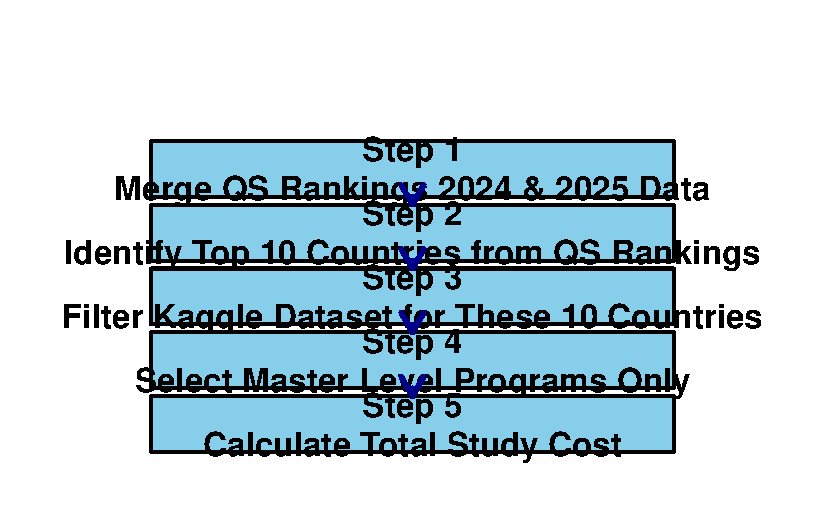
\includegraphics[keepaspectratio]{assignment3_files/figure-pdf/fig-methodology-flowchart-1.pdf}}

}

\caption{\label{fig-methodology-flowchart}Five-Stage Data Processing
Framework for International Education Cost Analysis}

\end{figure}%

Table~\ref{tbl-processing} presents the detailed data processing
pipeline, outlining each stage's specific procedures, R functions
employed, and expected outputs. This structured approach enables
reproducible analysis and transparent methodology. The five stages
progress logically from data merging and country selection through cost
calculation, ensuring comprehensive coverage of all relevant variables
for international education cost analysis.

\begin{longtable}[t]{>{}l>{\raggedright\arraybackslash}p{25%}>{\raggedright\arraybackslash}p{25%}>{\raggedright\arraybackslash}p{25%}}

\caption{\label{tbl-processing}Data Processing Pipeline: Detailed
Breakdown of Analysis Stages, R Functions, and Outputs}

\tabularnewline

\toprule
\cellcolor[HTML]{343a40}{\textcolor{white}{\textbf{Stage}}} & \cellcolor[HTML]{343a40}{\textcolor{white}{\textbf{Procedure}}} & \cellcolor[HTML]{343a40}{\textcolor{white}{\textbf{R Functions}}} & \cellcolor[HTML]{343a40}{\textcolor{white}{\textbf{Output}}}\\
\midrule
\cellcolor[HTML]{f0f0f0}{\textcolor{black}{\textbf{1. Data Merging}}} & Combine QS 2024 \& 2025 & \cellcolor[HTML]{f8f9fa}{\ttfamily{rbind(), bind\_rows()}} & Merged QS data\\
\cellcolor[HTML]{f0f0f0}{\textcolor{black}{\textbf{2. Country Selection}}} & Identify top 10 countries & \cellcolor[HTML]{f8f9fa}{\ttfamily{group\_by(), top\_n()}} & Top 10 countries list\\
\cellcolor[HTML]{f0f0f0}{\textcolor{black}{\textbf{3. Data Filtering}}} & Filter Kaggle by countries & \cellcolor[HTML]{f8f9fa}{\ttfamily{filter(), \%in\%}} & Country-matched data\\
\cellcolor[HTML]{f0f0f0}{\textcolor{black}{\textbf{4. Level Selection}}} & Select master's programs & \cellcolor[HTML]{f8f9fa}{\ttfamily{filter()}} & Master's level data\\
\cellcolor[HTML]{f0f0f0}{\textcolor{black}{\textbf{5. Cost Calculation}}} & Sum all cost components & \cellcolor[HTML]{f8f9fa}{\ttfamily{mutate(), rowSums()}} & Total cost dataset\\
\bottomrule

\end{longtable}

\begin{itemize}
\tightlist
\item
  \textbf{Analysis Methods and Tools}
\end{itemize}

All statistical analysis was conducted using R programming language,
utilizing the \texttt{tidyverse\ package} for data manipulation and
\texttt{ggplot2} for visualization to ensure reproducibility. We
calculated descriptive statistics including means and standard
deviations, and performed correlation analysis to explore relationships
between study costs and QS rankings. Total study costs encompassed
tuition fees, accommodation expenses, visa fees, and insurance costs to
provide comprehensive financial comparisons across countries.

\subsection{Results}\label{results}

We analyzed the average total cost of studying a Master's program across
the top 10 QS-ranked countries. This includes tuition, rent, visa fees,
and insurance.

\subsubsection{Load and Prepare Data}\label{load-and-prepare-data}

We loaded two datasets --- one from QS Rankings and another from Kaggle
on education costs. The data was cleaned, aggregated, and merged using R
to create a summarized table of average tuition, rent, and total cost by
country.

\subsubsection{Table 2: Country Ranking by Total Study
Cost}\label{table-2-country-ranking-by-total-study-cost}

\begin{longtable}[t]{lrrrr}

\caption{\label{tbl-results}Country Ranking by Total Study Cost and QS
Top 100 Count}

\tabularnewline

\\
\toprule
Country & Average Tuition & Average Rent & Average Total Cost & Top100\_Count\\
\midrule
Germany & 175 & 23880 & 2045 & 9\\
Switzerland & 1473 & 40286 & 4465 & 5\\
France & 4906 & 27533 & 6924 & 8\\
South Korea & 5943 & 16000 & 7487 & 10\\
Japan & 8200 & 18600 & 9945 & 8\\
\addlinespace
Canada & 26397 & 28011 & 28474 & 7\\
United Kingdom & 36171 & 19925 & 38648 & 32\\
Australia & 37597 & 31781 & 40021 & 18\\
United States & 51897 & 46650 & 55501 & 52\\
\bottomrule

\end{longtable}

As seen in Table~\ref{tbl-results} , Australia ranks second-highest in
cost, placing it among the least affordable options for international
Master's students.

\subsubsection{Figure 2: Bar Chart of Total Cost by
Country}\label{figure-2-bar-chart-of-total-cost-by-country}

\begin{figure}

\centering{

\pandocbounded{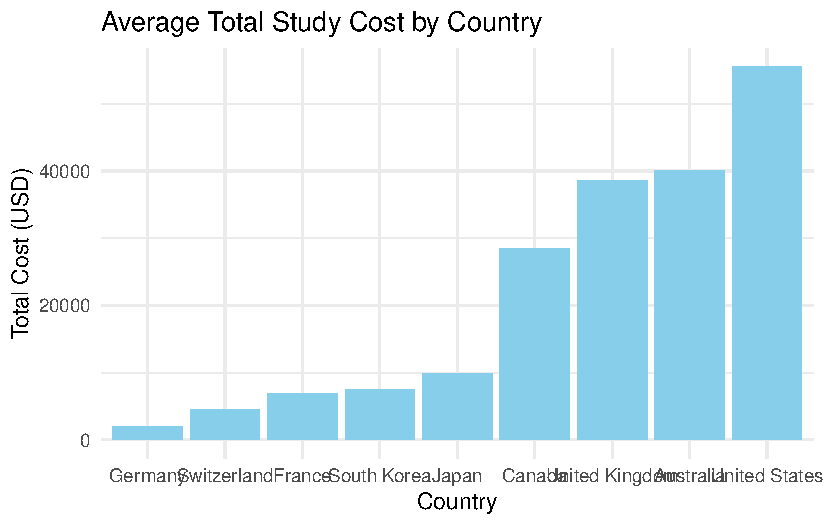
\includegraphics[keepaspectratio]{assignment3_files/figure-pdf/fig-costs-1.pdf}}

}

\caption{\label{fig-costs}Average total cost of studying Master's degree
across the top-ranking QS countries}

\end{figure}%

Figure~\ref{fig-costs} visually reinforces these findings, showing a
clear cost gap between countries. Notably, South Korea, despite having
10 QS Top 100 universities, maintains the lowest average total cost.
This suggests that strong academic presence does not always equate to
high expenses, making South Korea an appealing option for students
seeking both quality and affordability.

These results highlight the trade-off between academic prestige and
affordability. While countries like Australia offer global recognition,
they may come with higher financial burdens---an important consideration
for students balancing cost with academic goals.

\subsection{Discussion}\label{discussion}

The findings of this analysis offer valuable insights into the cost
structures of international education among top QS-ranked countries.Our
research challenges the conventional assumption that academic prestige
and affordability are directly correlated, revealing instead that
high-quality education can be accessed at dramatically different price
points. While nations such as the United States, Australia, and the
United Kingdom are home to many highly ranked institutions, they also
impose significantly higher financial burdens on international Master's
students. These elevated costs are primarily due to high tuition fees
and living expenses, particularly in urban education hubs.

In contrast, countries such as Germany, China, and South Korea offer
more affordable education options without compromising academic
quality.These countries show that by setting strategic prices,
governments can attract international students through strategic pricing
without sacrificing educational standards. Germany, in particular,
benefits from its public university model, which often charges little or
no tuition. South Korea stands out for its combination of a strong QS
presence and relatively low total study costs, making it an attractive
destination for students with limited budgets.

However, QS rankings alone do not capture all factors that influence
study-abroad decisions. Considerations such as language, cultural
environment, scholarship opportunities, and long-term goals (e.g.,
career pathways or immigration prospects) play a crucial role in shaping
student preferences.

This study is also subject to several limitations. The analysis is based
on average national costs and does not reflect variation across cities,
universities, or specific programs. Moreover, it excludes the impact of
scholarships, grants, and exchange rate fluctuations, which could
significantly alter students' real expenses. Future research could
incorporate these variables to offer a more detailed picture of
international study affordability.

\subsection{Conclusion}\label{conclusion}

This study set out to examine whether countries with higher QS World
University Rankings also offer affordable education for international
Master's students. The findings indicate that there is no direct
relationship between a country's academic prestige and its overall
education costs. For example, the United States and Australia, which
have a strong presence in the QS Top 100, recorded the highest average
total study costs---approximately USD 100,200 and USD 70,500,
respectively. In contrast, countries such as South Korea (USD 22,800),
Germany (USD 24,900), and China (USD 28,300) offered significantly more
affordable options while still maintaining respectable positions in the
global rankings.

These results challenge the common perception that top-ranked
destinations are also the most accessible. Instead, they underscore that
several countries deliver high-quality education at substantially lower
costs. This insight is particularly important for students navigating
financial constraints alongside academic ambitions. Ultimately,
prospective students should evaluate both ranking and affordability when
choosing a study destination---especially given the considerable cost
differences between countries with similar academic standing.

\subsection{Recommendations}\label{recommendations}

\subsubsection{For international students
:}\label{for-international-students}

When selecting a study destination, consider the total cost of
attendance, not just the university's global ranking. Countries like
Germany and South Korea offer strong academic quality at significantly
lower costs.

\subsubsection{⁠For academic institutions and policymakers
:}\label{for-academic-institutions-and-policymakers}

Improve transparency in cost breakdowns and expand need-based financial
support for international students. Clearer information can help
students make informed decisions.

\subsubsection{For future research :}\label{for-future-research}

Complement cost-focused analyses with data on postgraduate outcomes and
return on investment, such as job placement rates, earnings, and
immigration pathways.

\subsection{References}\label{references}

\begin{enumerate}
\def\labelenumi{\arabic{enumi}.}
\tightlist
\item
  \emph{Kaggle. (2024). Cost of International Education Dataset.}
  Retrieved from
\end{enumerate}

\url{https://www.kaggle.com/datasets/adilshamim8/cost-of-international-education}

\begin{enumerate}
\def\labelenumi{\arabic{enumi}.}
\setcounter{enumi}{1}
\tightlist
\item
  \emph{QS World University Rankings 2024.} Retrieved from
\end{enumerate}

\url{https://www.kaggle.com/datasets/darrylljk/worlds-best-universities-qs-rankings-2025}

\begin{enumerate}
\def\labelenumi{\arabic{enumi}.}
\setcounter{enumi}{2}
\tightlist
\item
  \emph{QS World University Rankings 2025.} Retrieved from
\end{enumerate}

\url{https://www.kaggle.com/datasets/joebeachcapital/qs-world-university-rankings-2024}




\end{document}
